\documentclass{article}

\usepackage[utf8]{inputenc}
\usepackage[brazil]{babel}
\usepackage{amsmath, amssymb}
\usepackage{graphicx}
\usepackage{hyperref}
\usepackage{float}
\usepackage{geometry}

\geometry{margin=1in}

\title{Mínimos Quadrados, ARX, ARMAX e OE}
\author{Eduardo Henrique Basilio de Carvalho}
\date{\today}

\begin{document}

\maketitle

\section*{Questão 1}

Seja

\begin{equation}
    y = 1.5x^2 + 0.7x - 2
\end{equation}

\subsection*{a}

A figura \ref{fig:parabola_sem_ruido} apresenta a curva para $x \in [-6, 6]$.

\begin{figure}[H]
    \centering
    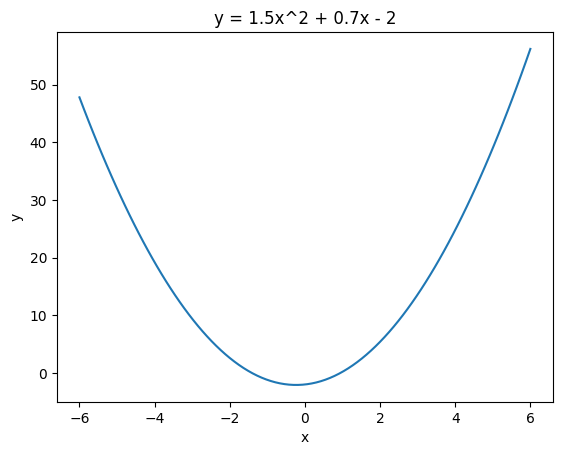
\includegraphics[width=0.7\textwidth]{imagens/parabola_sem_ruido.png}
    \caption{Curva de $y = 1.5x^2 + 0.7x - 2$}
    \label{fig:parabola_sem_ruido}
\end{figure}

\subsection*{b}

A figura \ref{fig:parabola_com_ruido} apresenta a curva com ruído uniforme com amplitude $\pm 0.1\text{max}(|y|)$.

\begin{figure}[H]
    \centering
    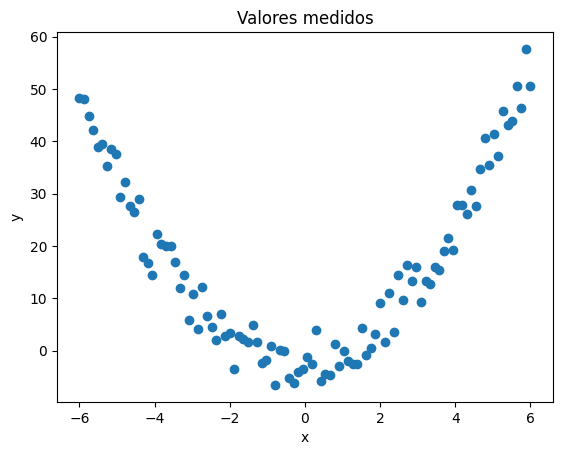
\includegraphics[width=0.7\textwidth]{imagens/parabola_com_ruido.png}
    \caption{Curva de $y = 1.5x^2 + 0.7x - 2$ com ruído}
    \label{fig:parabola_com_ruido}
\end{figure}

\subsection*{c}

A equação de regressão é $y = \theta_2x^2 + \theta_1x + \theta_0$.

\subsection*{d}

A matriz de regressores é

\begin{equation}
    A =
    \begin{bmatrix}
    x_1^2 & x_1 & 1 \\
    x_2^2 & x_2 & 1 \\
    \vdots & \vdots & \vdots \\
    x_N^2 & x_N & 1
    \end{bmatrix}
\end{equation}

\subsection*{e}

Os coeficientes estimados por mínimos quadrados são $\theta_0 = 1.52$, $\theta_1 = 0.47$ e $\theta_2 = -2.59$. A figura \ref{fig:parabola_referencia_vs_ajustada} compara a curva de referência com a obtida a partir dos parametrôs estimados.

\begin{figure}{H}
    \centering
    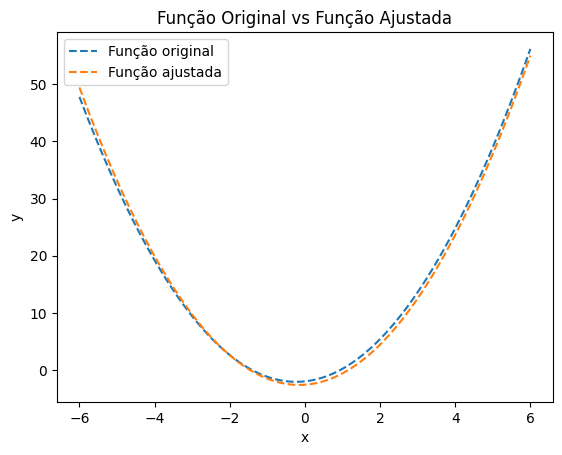
\includegraphics[width=0.7\textwidth]{imagens/parabola_referencia_vs_ajustada.png}
    \caption{Curva de referência vs curva ajustada}
    \label{fig:parabola_referencia_vs_ajustada}
\end{figure}

\subsection*{f}

Com 1000 pontos, a curva ajustada é $y = 1.51x^2 + 0.68x - 2.12$. A figura \ref{fig:parabola_referencia_vs_ajustada_N1000} compara a curva de referência com a obtida a partir dos parametrôs estimados.

\begin{figure}{H}
    \centering
    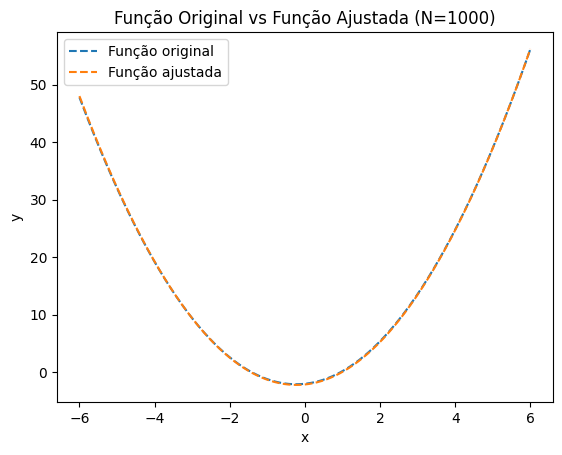
\includegraphics[width=0.7\textwidth]{imagens/parabola_referencia_vs_ajustada_N1000.png}
    \caption{Curva de referência vs curva ajustada para $N = 1000$}
    \label{fig:parabola_referencia_vs_ajustada_N1000}
\end{figure}

Com o aumento substancial de redundância, a estimação de parâmetros é mais robusta.

\subsection*{g}

Sob a soma de ruído com amplitude $0.1\Delta{x}$ na entrada, os coeficientes estimados são $\theta_0 = 1.25$, $\theta_1 = 0.66$ e $\theta_2 = 0.58$. A figura \ref{fig:parabola_referencia_vs_ajustada_Xruidoso_N1000} apresenta a curva correspondente.

\begin{figure}{H}
    \centering
    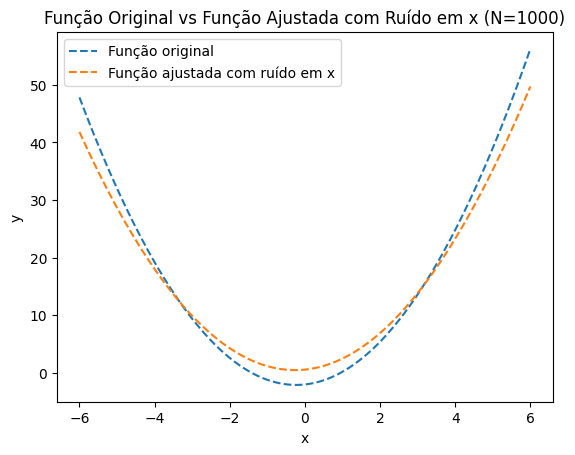
\includegraphics[width=0.7\textwidth]{imagens/parabola_referencia_vs_ajustada_Xruidoso_N1000.png}
    \caption{Curva de referência vs curva ajustada sob ruído na entrada (N=1000)}
    \label{fig:parabola_referencia_vs_ajustada_Xruidoso_N1000}
\end{figure}

Mesmo com a elevada quantidade de regressores, o ruído na entrada prejudica significativamente a estimação dos parâmetros.

\section*{Questão 2}

\subsection*{a, b, c, d}

A figura \ref{fig:sistemas_referencia} apresenta os sistemas simulados para uma mesma entrada.

\begin{figure}[H]
    \centering
    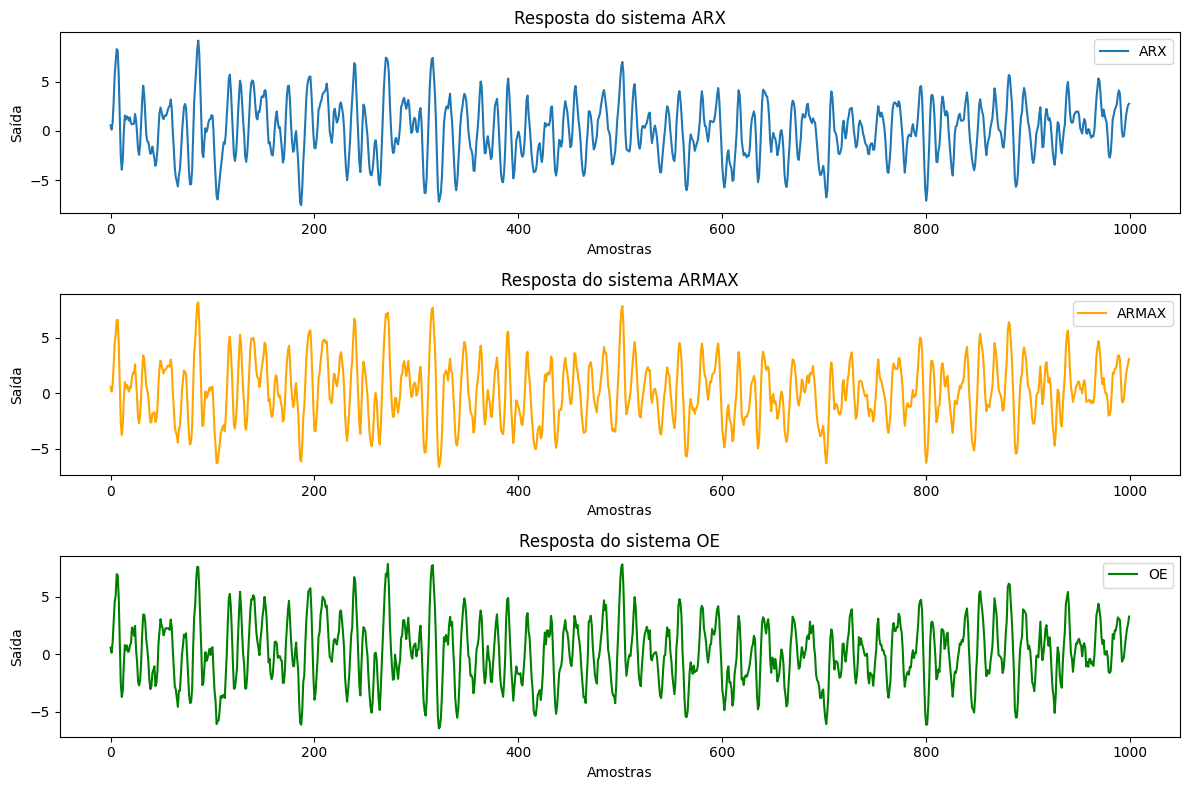
\includegraphics[width=0.7\textwidth]{imagens/sistemas_referencia.png}
    \caption{Sistemas de referência}
    \label{fig:sistemas_referencia}
\end{figure}

\section*{Questão 3}

\subsection*{ARX}

Dado

\begin{equation*}
    A(z)y[k] = B(z)u[k] + e[k]
\end{equation*}

com dois atrasos em $A(z)$ e $B(z)$,

\begin{align*}
    y[k]& + a_1y[k-1] + a_2y[k-2] = b_1u[k-1] + b_2u[k-2] + e[k] \\
    y[k]& = -a_1y[k-1] - a_2y[k-2] + b_1u[k-1] + b_2u[k-2] + e[k]
\end{align*}

Seja

\begin{align*}
    Y &=
    \begin{bmatrix}
    y[2] \\
    y[3] \\
    y[4] \\
    \vdots \\
    y[N-1]
    \end{bmatrix} \\
    \Phi &=
    \begin{bmatrix}
    y[1] & y[0] & u[1] & u[0] \\
    y[2] & y[1] & u[2] & u[1] \\
    y[3] & y[2] & u[3] & u[2] \\
    \vdots & \vdots & \vdots & \vdots \\
    y[N-2] & y[N-3] & u[N-2] & u[N-3]
    \end{bmatrix} \\
    \theta &=
    \begin{bmatrix}
    -a_1 \\
    -a_2 \\
    b_1 \\
    b_2
    \end{bmatrix} \\
    E &=
    \begin{bmatrix}
    e[2] \\
    e[3] \\
    e[4] \\
    \vdots \\
    e[N-1]
    \end{bmatrix}
\end{align*},

então

\begin{equation*}
    Y = \Phi\theta + E
\end{equation*}

e a estimativa por mínimos quadrados é

\begin{equation*}
    \hat{\theta} = (\Phi^T\Phi)^{-1}\Phi^TY
\end{equation*}

A figura \ref{fig:validacao_arx} compara a curva de referência com a curva ajustada por ARX. Ambas as respostas são computadas sobre um novo vetor de entrada, com as mesmas características do usado para a estimação, mas em outra realização, a fim de confirmar generalização.

\begin{figure}[H]
    \centering
    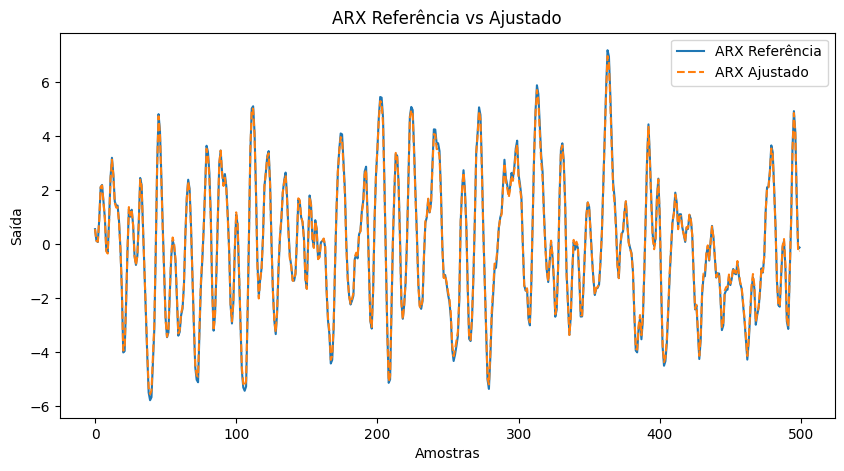
\includegraphics[width=0.7\textwidth]{imagens/validacao_arx.png}
    \caption{Curva de referência vs curva ajustada por ARX}
    \label{fig:validacao_arx}
\end{figure}

\subsection*{ARMAX}

Dado

\begin{equation*}
    A(z)y[k] = B(z)u[k] + C(z)e[k]
\end{equation*}

com dois atrasos em $A(z)$, $B(z)$ e $C(z)$,

\begin{align*}
    y[k]& + a_1y[k-1] + a_2y[k-2] = b_1u[k-1] + b_2u[k-2] + e[k] + c_1e[k-1] + c_2e[k-2] \\
    y[k]& = -a_1y[k-1] - a_2y[k-2] + b_1u[k-1] + b_2u[k-2] + e[k] + c_1e[k-1] + c_2e[k-2]
\end{align*}

A construção

\begin{equation*}
    Y = \Phi\theta
\end{equation*}

com

\begin{align*}
    Y &=
    \begin{bmatrix}
    y[2] \\
    y[3] \\
    y[4] \\
    \vdots \\
    y[N-1]
    \end{bmatrix} \\
    \Phi &=
    \begin{bmatrix}
    y[1] & y[0] & u[1] & u[0] & e[1] & e[0] \\
    y[2] & y[1] & u[2] & u[1] & e[2] & e[1] \\
    y[3] & y[2] & u[3] & u[2] & e[3] & e[2] \\
    \vdots & \vdots & \vdots & \vdots & \vdots & \vdots \\
    y[N-2] & y[N-3] & u[N-2] & u[N-3] & e[N-2] & e[N-3]
    \end{bmatrix} \\
    \theta &=
    \begin{bmatrix}
    -a_1 \\
    -a_2 \\
    b_1 \\
    b_2 \\
    c_1 \\
    c_2
    \end{bmatrix}
\end{align*}

é valida, mas não pode ser usada para estimar $\theta$ por mínimos quadrados, pois $e[k]$ não é conhecido. Neste caso, o método *quadrados mínimos extendido* é uma solução. O algoritmo é:

1. Estime um modelo ARX sobre os dados;
2. Calcule os resíduos do modelo ARX estimado;
3. Use os resíduos como uma estimativa para $e[k]$ e construa a matriz de regressores;
4. Estime o modelo ARMAX usando mínimos quadrados;
5. Calcule os resíduos do modelo ARMAX estimado;
6. Repita os passos 3 a 5 até convergência.

A figura \ref{fig:validacao_armax} compara a curva de referência com a curva ajustada por ARMAX. As condições para o vetor de validação são as mesmas da validação do ARX.

\begin{figure}[H]
    \centering
    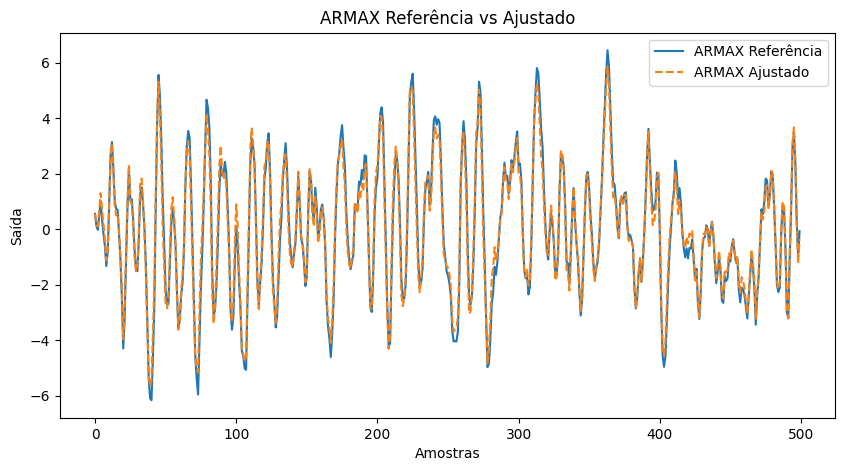
\includegraphics[width=0.7\textwidth]{imagens/validacao_armax.png}
    \caption{Curva de referência vs curva ajustada por ARMAX}
    \label{fig:validacao_armax}
\end{figure}

\subsection*{OE}

Dado

\begin{equation*}
    F(z)y[k] = B(z)u[k] + F(z)e[k]
\end{equation*}

com dois atrasos em $F(z)$ e $B(z)$,

\begin{align*}
    y[k]& + f_1y[k-1] + f_2y[k-2] = b_0u[k] + b_1u[k-1] + b_2u[k-2] + f_0e[k] + f_1e[k-1] + f_2e[k-2] \\
    y[k]& = -f_1y[k-1] - f_2y[k-2] + b_0u[k] + b_1u[k-1] + b_2u[k-2] + f_0e[k] + f_1e[k-1] + f_2e[k-2]
\end{align*}

Assim como para ARMAX, a separação entre saída, regressores e parâmetros constrói um sistema não linear nos parâmetros. Porém, neste caso, não é possível partir de uma estimativa inicial que ignore os erros de medição, já que assumir $F(z) = 1$ desconsidera, também, a dinâmica do sistema. Resta, então, resolver por otimização não linear. Um algoritmo candidato é:

1. Estime F como A em um modelo ARX (chute inicial);
2. Compute B correspondente, dado que y, u e F são conhecidos, assim como e, assumido zero;
3. Calcule os resíduos do modelo OE estimado;
4. Compute um novo F, minimizando os resíduos;
5. Repita os passos 2 a 4 até convergência.

A figura \ref{fig:validacao_oe} compara a curva de referência com a curva ajustada por OE. As condições para o vetor de validação são as mesmas da validação do ARX.

\begin{figure}[H]
    \centering
    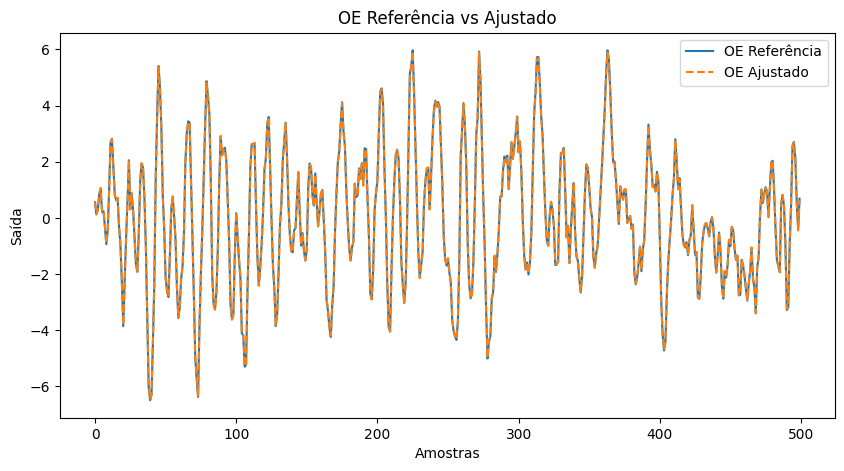
\includegraphics[width=0.7\textwidth]{imagens/validacao_oe.png}
    \caption{Curva de referência vs curva ajustada por OE}
    \label{fig:validacao_oe}
\end{figure}

\subsection*{Comparação}

\subsubsection*{ARX}

A identificação foi simples e resultou em um modelo com boa performance na validação. Isso decorre de ser um modelo totalmente linear nos parametros desde o princípio, o que permite o uso direto de mínimos quadrados.

\subsubsection*{ARMAX}

A identificação ainda é consideravelmente simples, dado que estimar os erros é um problema de regressão linear. Assim como o ruído filtrado é a diferença entre a saída medida e a resposta da função geradora, os resíduos são a diferença entre a saída medida e a resposta do modelo estimado. Por isso, este é um estimador adequado para aquele. A performance decorrente dessa consideração, no entanto, foi inferior à dos demais casos.

\subsubsection*{OE}

Descartada a possibilidade de regressão linear, a identificação é mais complexa. Tal complexidade, entretanto, é concentrada na seleção de um novo candidato para F, passo que pode ser delegado ao módulo SciPy. Com esta ferramenta mais robusta, a performance do modelo foi, visualmente, tão boa quanto a do ARX.

\section*{Questão 4}

Seja $J_{MQ}=(y-\Psi\Theta)^{T}(y-\Psi\Theta)$ e $\Psi$ não singular.

\begin{align*}
    J_{\text{reg}}&=\tfrac12\big[(y-\Psi\Theta)^{T}(y-\Psi\Theta)\big]+\tfrac12\lambda\Theta^{T}\Theta \\
    J_{\text{reg}}&=\tfrac12(y^{T}y-2y^{T}\Psi\Theta+\Theta^{T}\Psi^{T}\Psi\Theta)+\tfrac12\lambda\Theta^{T}\Theta \\
    \nabla_{\Theta}J_{\text{reg}}&=-\Psi^{T}y+(\Psi^{T}\Psi)\Theta+\lambda\Theta \\
\end{align*}

Para ponto crítico,

\begin{gather*}
    0=-\Psi^{T}y+(\Psi^{T}\Psi)\Theta+\lambda\Theta \\
    (\Psi^{T}\Psi+\lambda I)\Theta=\Psi^{T}y \\
    \hat\Theta_{\text{reg}}=(\Psi^{T}\Psi+\lambda I)^{-1}\Psi^{T}y
\end{gather*}

Para mínimo,

\begin{equation*}
    \nabla^{2}_{\Theta}J_{\text{reg}}=\Psi^{T}\Psi+\lambda I>0
\end{equation*}

O que é garantido para $\lambda>0$.


\end{document}
